\chapter{Practice Exam 2}
    Michael is designing a motor driver for a wheeled mobile robot. The motor driver is designed as
    an inverting amplifier (using the circuit shown in Figure 1) to drive the motor in the opposite
    direction of the input voltage. Michael would like to select the components of the amplifier
    based on specific design requirements. Michael has installed a switch ($Sw_1$) to disconnect the
    motor driver input signal ($v_{in}$) to the system and a motor protection switch ($Sw_2$) to disconnect
    the motor from the amplifier when the motor is not used. A simplified model of a DC motor has
    been used, made up of a resistor and inductor in series. The DC motor generates a torque
    proportional to the current ($i_{out}$) through the inductor
    \begin{figure}[H]
        \centering
        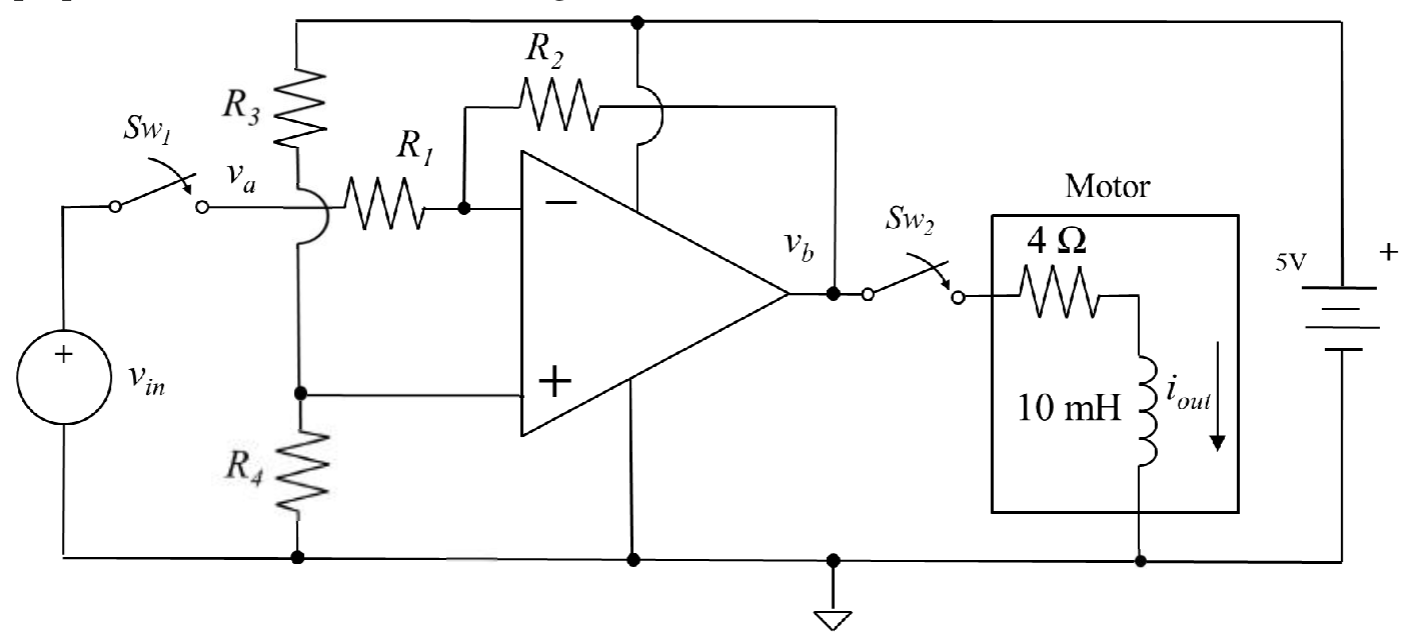
\includegraphics[width=0.6\linewidth]{figures/exams/motor_amp.png}
    \end{figure}
    \begin{enumerate}
        \item Design an inverting amplifier by choosing suitable resistor values for R1 and R2 to
        produce a gain of 5 when both switches Sw1 and Sw2 are open.\\
            \textbf{Solution:}\\
            \begin{minipage}{0.6\linewidth}
                \begin{figure}[H]
                    \centering
                    \begin{circuitikz}[american]
                        % op amp inverting 
                        \draw (0,0) node[op amp] (opamp) {};
                        \draw (opamp.-)
                            to[short, -*] ++(0,1);
                        \draw (opamp.+)
                            to[short, -*] ++(0,-2);
                        % circuit
                    \end{circuitikz}
                \end{figure}
            \end{minipage}
            \begin{minipage}{0.3\linewidth}
                \begin{flalign*}
                    \left|\text{Gain}\right| = \left|-\frac{R_2}{R_1}\right| &= 5\\
                    \text{Let } R_1 &= 1k\Omega\\
                    \therefore R_2 &= 5k\Omega
                \end{flalign*}
            \end{minipage}\\
        \item Design the bias input circuit by choosing suitable resistors R3 and R4 such that the
        voltage $v_b$ will be 0.5V if the positive power supply of the op-amp is connected to a 5V
        battery. Again both switches are open.\\
            \textbf{Solution:}\\
                    \begin{figure}[H]
                        \centering
                        \begin{circuitikz}[american]
                            \draw (0,0)
                                to[resistor, R=R3] (0,2.5)
                                to[resistor, R=R4] (0,5)
                                to[short] (5,5)
                                to[voltage source, v<=5V] (5,1)
                                to[short] (5,0)
                                to[short] (0,0);
                            \draw (2.5,3) node[op amp] (opamp) {};
                            \draw (opamp.up)
                                to[short, -*] ++(0,1.45);
                            \draw (opamp.down)
                                to[short, -*] ++(0,-2.45);
                            \draw (opamp.+) to[short, -*] ++(-1.3,0);
                        \end{circuitikz}
                    \end{figure}    
                    By removing the op amp as its outputs aren't connected we can identify that it is in
                    a voltage divider configuration
                \begin{minipage}{0.6\linewidth}
                    \begin{figure}[H]
                        \centering
                        \begin{circuitikz}[american]
                            \draw (0,0)
                                to[voltage source, v=5V, invert] (0,4)
                                to[short] (2,4)
                                to[resistor, R=R1] (2,2)
                                to[resistor, R=R2] (2,0)
                                to[short] (0,0);
                            \draw (2,2)
                                to[short] (4,2)
                                to[open] (4,0)
                                to[short] (2,0);
                            \node at (4,1) {$v_{out}$};
                            \draw [->] (4,0.8) -- (4,0.1);
                            \draw [->] (4,1.1) -- (4,1.8);
                        \end{circuitikz}
                    \end{figure}
                \end{minipage}
                \begin{minipage}{0.3\linewidth}
                    \begin{flalign*}
                        v_{out} &= \frac{R_2}{R_1 + R_2} v_{in}\\
                        0.5 &= \frac{R_2}{R_1 + R_2} 5\\
                        0.1 &= \frac{R_2}{R_1 + R_2}\\
                        10(R_1 + R_2) &= R_2\\
                        \text{Let } R_1 &= 1k\Omega\\
                        \therefore R_2 &= 9k\Omega
                    \end{flalign*}
                \end{minipage}
        \item Given $Sw_1$ is open, the amplifier is turned on for enough time, such that the voltages
        stabilise, Michael connects the motor by closing Sw2 and the motor starts to move. Find
        the step response of the motor current, iout. Assume that the amplifier output resistance is
        negligible, it does not current limit and the motor inductor has been de-energised\\
            \textbf{Solution:}\\
        \item What is the steady state voltage across the motor?\\
            \textbf{Solution:}\\
        \item Perform frequency response analysis from vin, to the voltage across the motor inductor,
        when both switches are closed and Michael applies three different input signals of 10 Hz,
        100 Hz and 1000 Hz through the system?
            \textbf{Solution:}\\
        \item Plot the response calculated in part (e) in a Bode plot\\
            \textbf{Solution:}\\
    \end{enumerate}